\documentclass[border=125pt,tikz]{standalone}
\usetikzlibrary{arrows.meta,automata,positioning}

\begin{document}

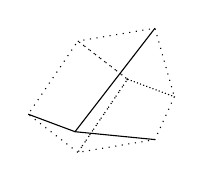
\begin{tikzpicture}
\pgfmathsetmacro{\cubex}{1}
\pgfmathsetmacro{\cubey}{1}
\pgfmathsetmacro{\cubez}{1}


\draw[black] (0,0,1.732) -- (-0.8165,0,1.155) -- (0,0,1.732) -- (0.408,0.7071,0.155) -- (0,0,1.732) -- (0.408,-0.7071,0.155);

\draw[black,dotted] (0,0,0) -- (0.8165,0,0.5773) -- (0.408,0.7071,0.155) -- (-0.408,0.7071,0.5773) -- cycle;
\draw[black,dotted] (0,0,0) -- (-0.408,0.7071,0.5773) -- (-0.8165,0,1.155) -- (-0.408,-0.7071,0.5773) -- cycle;
\draw[black,dotted] (0,0,0) -- (-0.408,-0.7071,0.5773) -- (0.408,-0.7071,0.155) -- (0.8165,0,0.5773) -- cycle;


\end{tikzpicture}

\end{document}
